\documentclass[autodetect-engine,dvipdfmx-if-dvi,ja=standard]{bxjsarticle}

% 二段組にするとき
% \documentclass[twocolumn,autodetect-engine,dvipdfmx-if-dvi,ja=standard]{bxjsarticle}

\usepackage{graphicx}        %図を表示するのに必要
\usepackage{color}           %jpgなどを表示するのに必要
\usepackage{amsmath,amssymb} %数学記号を出すのに必要
\usepackage{setspace}
\usepackage{eclclass}
\usepackage{cases}
\usepackage{here}
\usepackage{fancyhdr}
\usepackage{ascmac}

% 文書全体のスタイルを設定(主に余白)
\setlength{\topmargin}{-0.3in}
\setlength{\oddsidemargin}{0pt}
\setlength{\evensidemargin}{0pt}
\setlength{\textheight}{44\baselineskip}

% 行頭の字下げをしない
\parindent = 0pt

% ヘッダとフッタの設定
\lhead{電気情報工学応用実験II}
\chead{}
\rhead{5E 20番 佐藤凌雅}
\lfoot{}
\cfoot{-\thepage-} % ページ数
\rfoot{}

% 式の番号を(senction_num.num)のようにする
\makeatletter
\@addtoreset{equation}{section}
\def\theequation{\thesection.\arabic{equation}}
\makeatother

% 画像の貼り付けを簡単にする
\newcommand{\pic}[2]
{
  \begin{figure}[H]
    \begin{center}
      \includegraphics[scale=#2]{#1}
    \end{center}
  \end{figure}
}

% 単位の記述を簡単にする
\newcommand{\unit}[1]
{
  \, [\mathrm{#1}]
}
\begin{document}
% \maketitle
\pagestyle{fancy}

\section{目的}
 マイクロ波回路の立体回路(波導管,マジックT)の特性とマイクロ波ホーンアンテナによる伝送の仕組みを実験により理解する.

\section{予習}
・マイクロ波発生装置である反射型クライストロンとガンダイオード発振器について調べよ.\\
 クライストロンとは,マイクロ波用真空管の一種で,速度変調管とも呼ばれる.その中でも,反射形クライストロンは発振専用のものであり,空洞共振器を単独で使い,一つの共振器を高周波電場の入力と出力として同時に用いて反射電極で電子を逆行させて共振によるマイクロ波を発生させる.\footnote{真空管[クライストロン]物語\\http://kawoyama.la.coocan.jp/tubestoryklystron.html,2019-5-27閲覧}\\
 ガンダイオードは,ガリウム砒素(GaAs)の半導体に高電圧をかけたときに振動電流が発生するガン効果を利用した,マイクロ波発振素子.通常のダイオードがP型半導体とN型半導体から構成されるのに対し,ガン・ダイオードはN型半導体のみにより構成される.\footnote{ガンダイオード(Gunn diode):一口メモ\\http://mh.rgr.jp/memo/sc0035.htm,2019-5-27閲覧}\\

・マイクロ波回路のアイソレータ,クリスタルマウント,マジックTについて構造や動作原理を調べよ.\\
アイソレータ:アンプ(増幅器)の後段に配置することにより,折り返しがアンプ(増幅器)の出力ポートに戻らないよう遮断,アンプ(増幅器)を保護する部品.\footnote{サーキュレータ・アイソレータ | エム・アールエフ\\https://www.mrf.co.jp/product/ferrite\_circulator/,2019-5-27閲覧}\\
クリスタルマウント:マイクロ波検出用のダイオード.交流マイクロ波信号を直流に変換する整流機能を有する.\footnote{マイクロ波-アリオス株式会社-\\https://www.arios.co.jp/library/p16.html,2019-5-27閲覧}\\
マジックT:マジックT型導波管は,分岐が電界面に平行に出るE面T分岐導波管と磁界面に平行にでるH面T分岐導波管を組み合わせた導波管.\footnote{マジックT型導波管の電磁波解析 - ITアシストコム\\http://www.it-ac.co.jp/fw1002/fw0103/dx0111.html,2019-5-27閲覧}\\

\section{概要}
 高周波伝送には一般に同軸ケーブルが使用されるがマイクロ波の周波数では表皮効果による損失が大きいため断面寸法比が2:1の方形導波管が使用される.
 導波管は長辺の寸法aの二倍の長さに等しい遮断波長$\lambda_c$を持ち,広域通過フィルタの特性をもつ.

\section{実験手順\label{jikken}}
\begin{enumerate}
    \item 定常波測定器にクリスタルマウントをクリップで接続する.マイクロ波発振専用電源のMOD SELECTORをCWにし電源投入後,電源電圧計が9Vであることを確認する.
    クリスタルマウントの出力を測定し,マイクロ波の発生を確認する.

    \item 空洞周波数計のつまみを時計方向に回しきった状態から反時計方向に回転させ,クリスタルマウントが最小となる点を探す.周波数校正図から発信周波数を求める.
    \item クリスタルマウントの接続部に指定された長方形穴のあいた金属板を挟んだ場合の発振強度を測定し,1の場合と比較する.

    \item 定在波測定器にマジックTの各断面を接続し,他の3個の断面に向反射終端器2個とクリスタルマウントを接続する.各面のマイクロ波強度を測定し,マジックTの電装特性を調査する.

    \item マイクロ波発振機専用電源のMOD SELECTORをINTに切り替える.この時,マイクロ波は1kHzの方形波を変調信号とする振幅変調がかかっている.クリスタルマウントから方形波が出力されていることをオシロスコープで観測し,波形をスケッチする.

    \item 定在波測定器とクリスタルマウント間にマイクロホーン(電波ラッパ)を取り付け,空間伝送による送受信が可能であるか確認し出力波形をスケッチする.その後,受信アンテナの角度を正面に対して5度間隔で変化させてアンテナ指向性を測定し,グラフ化する.
  \end{enumerate}

  \newpage

  \section{使用機器\label{kiki}}
  \subsection{金属板}
  実験\ref{jikken}.3で使用した金属板の画像を図1から図6に示す.

  \begin{figure}[htpb]
    \centering

  \begin{tabular}{c}
    \begin{minipage}{0.50\hsize}
    \centering
    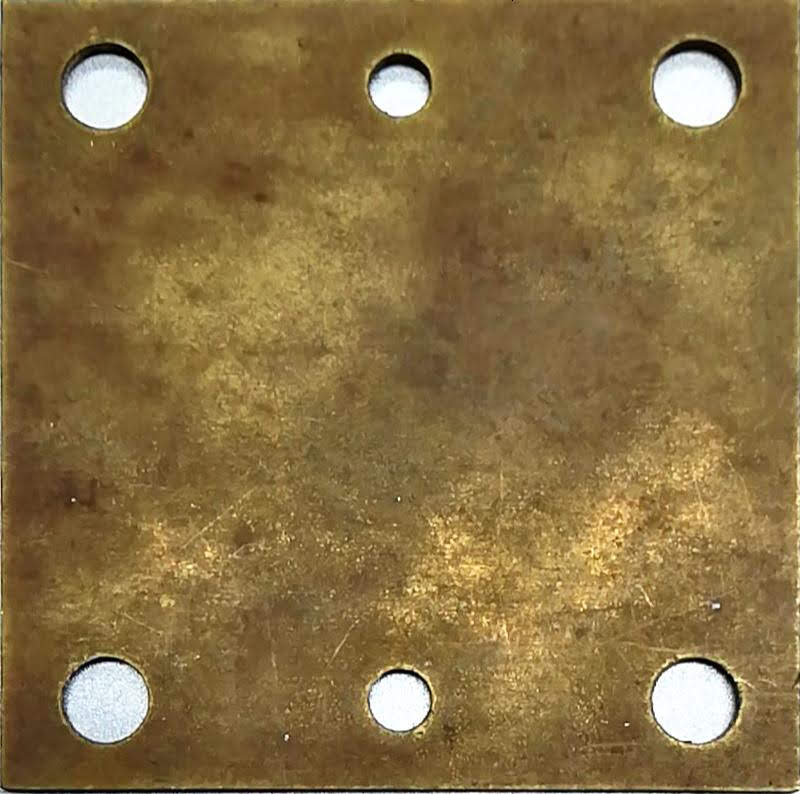
\includegraphics[keepaspectratio, width=4cm]{./data/1.png}
    \caption{}
    \end{minipage}

    \begin{minipage}{0.50\hsize}
    \centering
    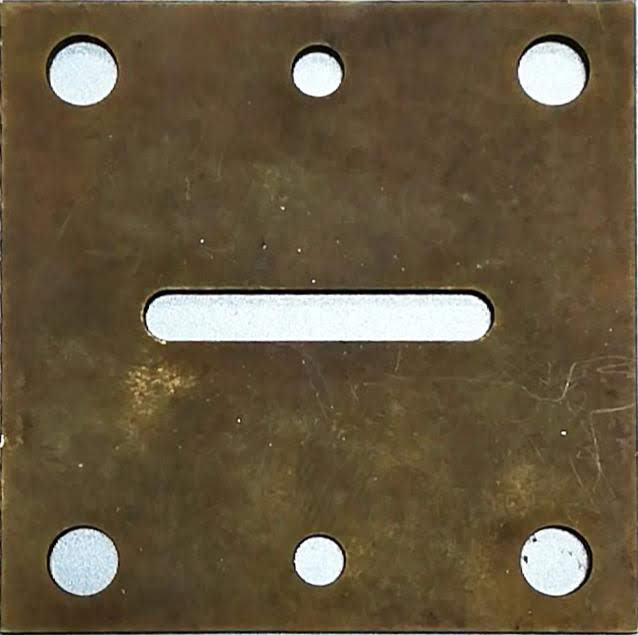
\includegraphics[keepaspectratio, width=4cm]{./data/2.png}
    \caption{}
    \end{minipage}

    \\
    \\
    \begin{minipage}{0.50\hsize}
    \centering
    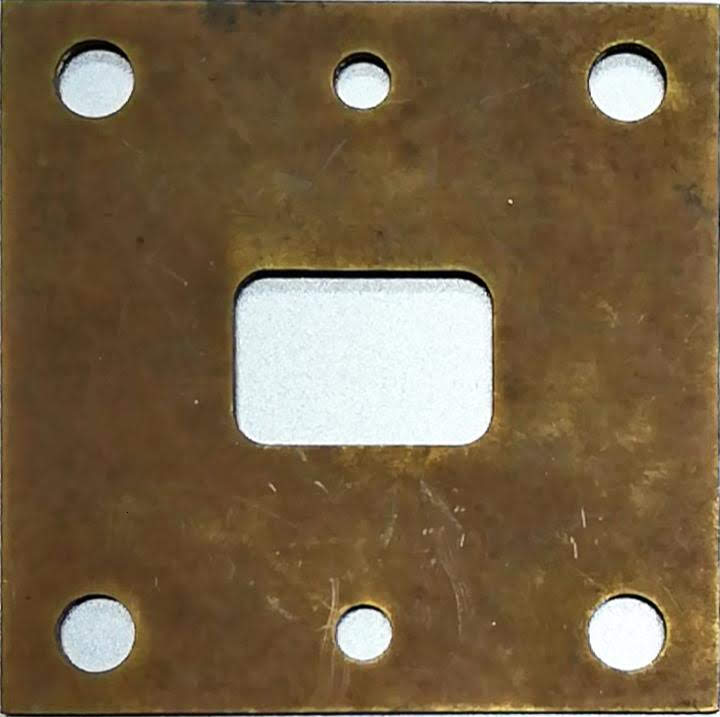
\includegraphics[keepaspectratio, width=4cm]{./data/3.png}
    \caption{}
    \end{minipage}

    \begin{minipage}{0.50\hsize}
    \centering
    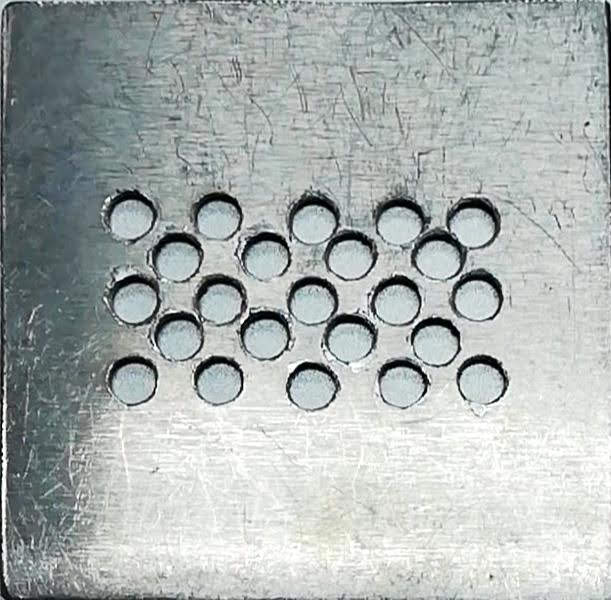
\includegraphics[keepaspectratio, width=4cm]{./data/4.png}
    \caption{}
    \end{minipage}

    \\
    \\

    \begin{minipage}{0.50\hsize}
      \centering
      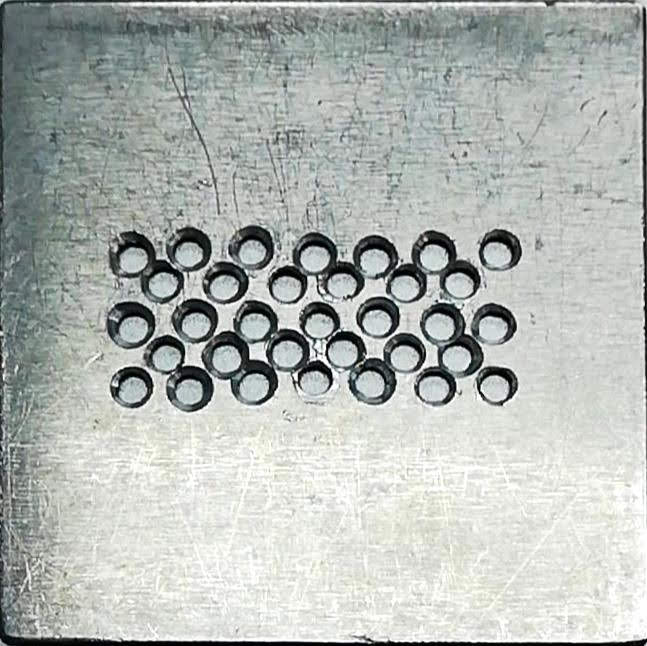
\includegraphics[keepaspectratio, width=4cm]{./data/5.png}
      \caption{}
      \end{minipage}

      \begin{minipage}{0.50\hsize}
      \centering
      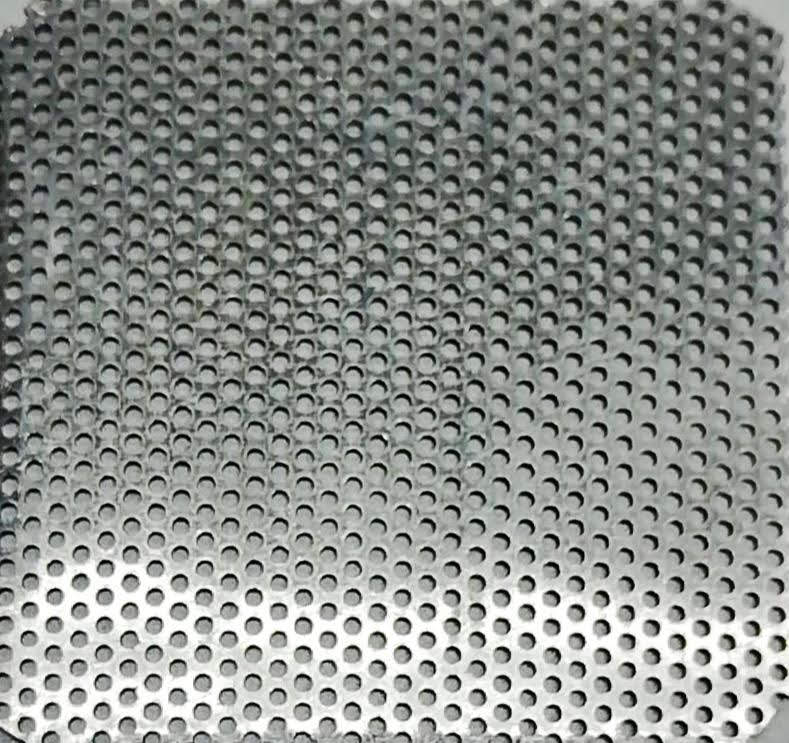
\includegraphics[keepaspectratio, width=4cm]{./data/6.png}
      \caption{}
      \end{minipage}
  \end{tabular}
\end{figure}

\subsection{金属板}
実験\ref{jikken}.3で使用したマジックTの画像を図7に示す.
\begin{figure}
  \centering
  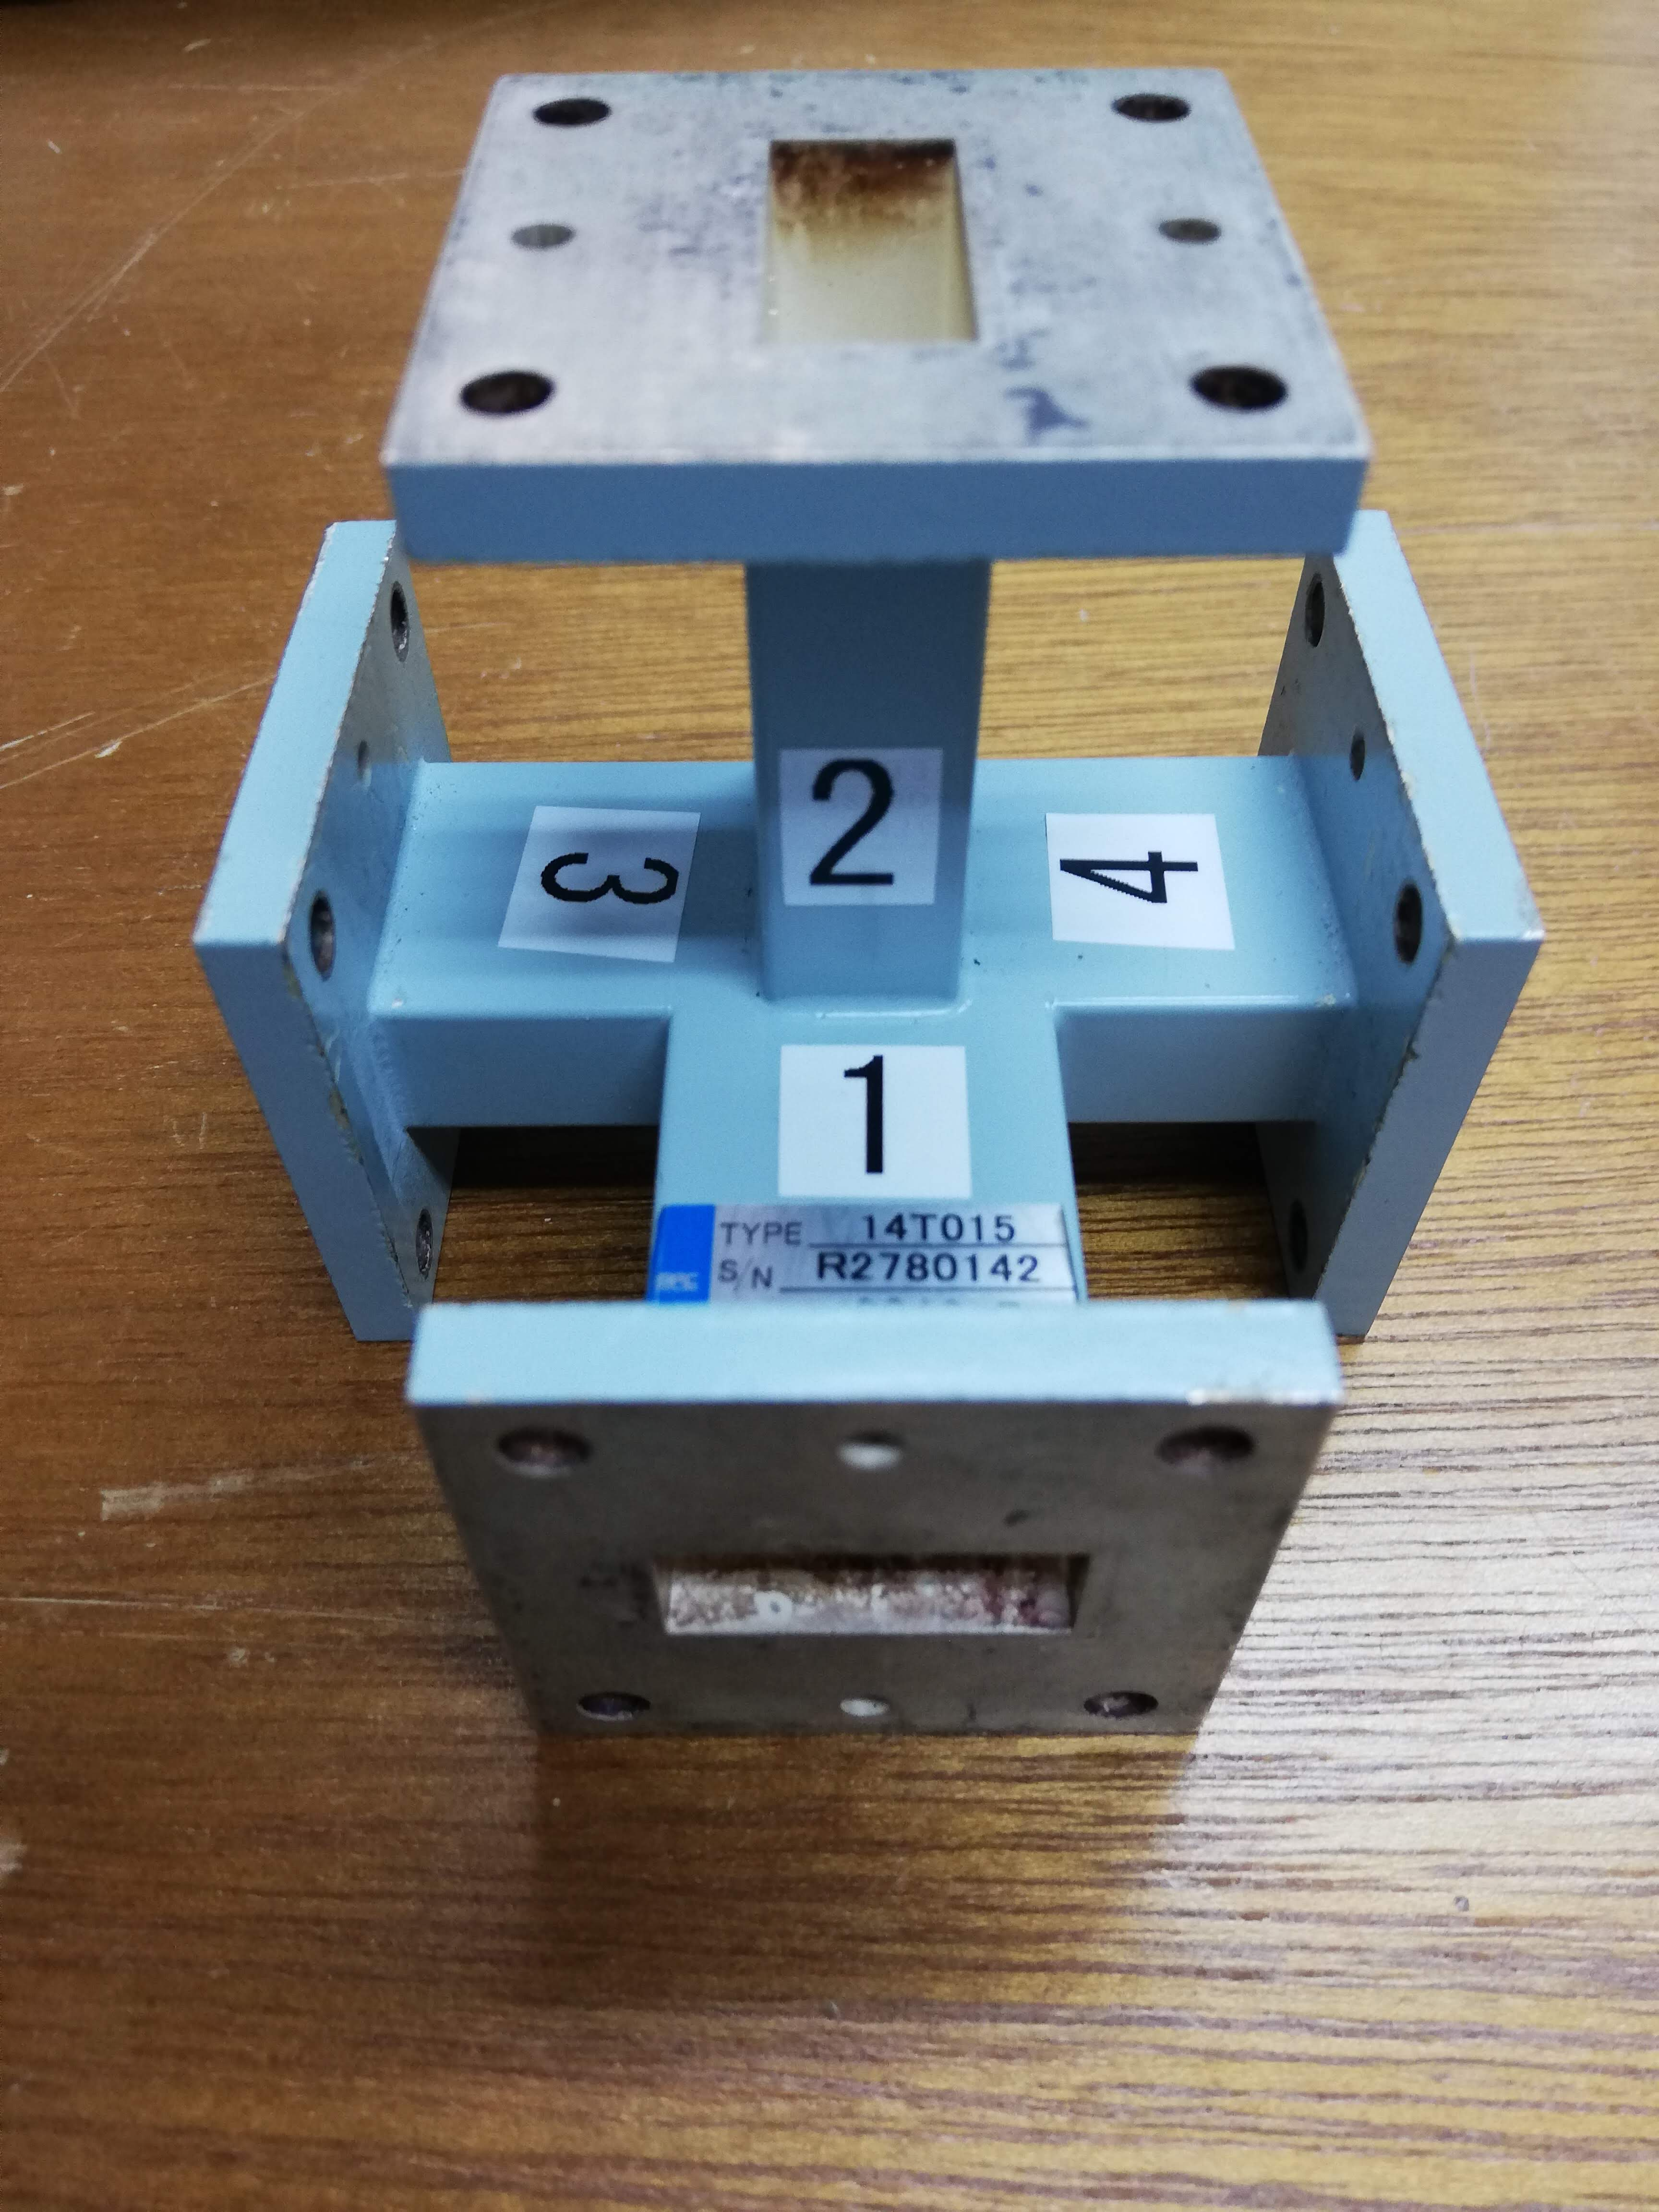
\includegraphics[width=5cm]{./data/magicT.jpg}
  \caption{マジックT}
\end{figure}

\newpage


\section{実験結果}
\subsection{実験\ref{jikken}.1}
 発振器の電源を投入したところ,電圧計は9Vを示した.また,クリスタルマウントの出力からマイクロ波の発生が確認できた.

\subsection{実験\ref{jikken}.2}
 クリスタルマウントの出力が最小となる点は3.01mmであった.周波数校正図から9338MHzであることが確認できた.

\subsection{実験\ref{jikken}.3}
 金属板を挟んだ場合のそれぞれの発振強度を表1に示す.表内の図番号は \ref{kiki}使用機器 と一致している.

  \begin{table}[H]
    \caption{金属板を挟んだ場合の発振強度}
    \centering
      \begin{tabular}{|l|l|}
      \hline
      金属板 & 発振強度   \\ \hline
      図1  & 0uV    \\ \hline
      図2  & 2.22V  \\ \hline
      図3  & 1.36V  \\ \hline
      図4  & 32mV   \\ \hline
      図5  & 5.2mV  \\ \hline
      図6  & 0.86mV \\ \hline
    \end{tabular}
  \end{table}

  \subsection{実験\ref{jikken}.4}
   定在波測定器にマジックTの各断面を接続し,他の3個の断面に向反射終端器2個とクリスタルマウントを接続した場合の各面のマイクロ波強度を表2に示す.この時のマジックTの断面番号は図7の写真と一致している.

  \begin{table}[H]
    \centering
    \caption{マジックTを接続した場合のマイクロ波強度}
    \begin{tabular}{cl|l|l|l|l|}
    \cline{3-6}
    \multicolumn{1}{l}{}                      &   & \multicolumn{4}{c|}{出力}       \\ \cline{3-6}
    \multicolumn{1}{l}{}                      &   & 1     & 2     & 3     & 4     \\ \hline
    \multicolumn{1}{|c|}{\multirow{4}{*}{入力}} & 1 &    -   & 1.1mV & 1.3V  & 1.28V \\ \cline{2-6}
    \multicolumn{1}{|c|}{}                    & 2 & 0.4mV &   -    & 1.3V  & 1.3V  \\ \cline{2-6}
    \multicolumn{1}{|c|}{}                    & 3 & 1.2V  & 1.2V  &    -   & 160mV \\ \cline{2-6}
    \multicolumn{1}{|c|}{}                    & 4 & 1.2V  & 1.2V  & 170mV &   -    \\ \hline
    \end{tabular}
  \end{table}

  \subsection{実験\ref{jikken}.5}
   オシロスコープで観測された方形波を図8に示す.

  \subsection{実験\ref{jikken}.6}
   空間伝送による出力波形を図9に示す.また,アンテナ指向性の測定結果を表3と図10に示す.
  \begin{table}[H]
    \centering
    \caption{ホーンアンテナ指向性}
    \begin{tabular}{|l|l|}
    \hline
    角度{[}deg{]} & 発振強度{[}mV{]} \\ \hline
    0           & 555          \\ \hline
    5           & 515          \\ \hline
    10          & 440          \\ \hline
    15          & 322          \\ \hline
    20          & 237          \\ \hline
    25          & 161          \\ \hline
    30          & 105          \\ \hline
    35          & 53.3         \\ \hline
    40          & 37.0         \\ \hline
    45          & 14.1         \\ \hline
    50          & 5.0          \\ \hline
    55          & 5.0          \\ \hline
    60          & 1.5          \\ \hline
    65          & 1.0          \\ \hline
    70          & 2.4          \\ \hline
    75          & 2.1          \\ \hline
    80          & 1.9          \\ \hline
    85          & 2.1          \\ \hline
    90          & 1.4          \\ \hline
    \end{tabular}
  \end{table}

  \end{document}
